\chapter{Aufgaben}
    \section{Berechnung der Schaltung}
        \subsection{Berechnung der Arbeitspunkte A, B und C}
            \paragraph{Arbeitspunkt A} Bei der Berechnung der Spannung \(U_A\) im Punkt \textbf{A} kann man den Spannungsteiler verwenden.
            Hier bei kam folgendes Ergebnis raus: 
            \begin{align*}
                U_A & = U_{V_2}\frac{R_2}{R_1+R_2} \\
                 & = 20\,V\frac{33k\,\Omega }{220k\,\Omega+33k\,\Omega}\\
                 & = 2,609\,V
            \end{align*}
            \paragraph{Arbeitspunnt B} Für die Berechnung der Spannung \(U_B\) im Punkt \textbf{B} betrachtet man den Spannungsabfall zwischen Punkt \textbf{A} und der Erdung in der Schaltung.
            Die Spannung am Widerstand \(R_4\) ist gleich der Spannung am Punkt \textbf{B}. Damit ergibt sich folgende Funktion.
            \begin{equation*}
                U_A = U_{BE} + U_B + U_{R_5}
            \end{equation*}
            Da Der Basisstrom vernachlässigt und man annimmt das der Kollektorstrom ungefähr gleich dem Emitterstrom ist, ergibt sich für \(U_{R_5} = I_C \cdot R_5\).
            \begin{equation}
                \label{ua}
                U_A = U_{BE} + U_B + I_C \cdot R_5
            \end{equation}
            Die Berechnung des Kollektorstrom läuft dann wie folgt. 
            \begin{align*}
                I_E\approx I_C & = \frac{U_B-U_{BE}}{R_5+R_4}\\
                &=\frac{2,609\,V-0,65\,V}{1k\,\Omega +2,2k\,\Omega}\\
                &=0,612m \,A
            \end{align*}
            Durch einsetzen und umstellen der Gleichung~\ref{ua} ergibt sich folgendes
            \begin{align*}
                U_B & = U_A-U_{BE}-I_C\cdot R_5\\
                & = 2,609\,V-0,65\,V-0,612m\,A\cdot 1k\,\Omega\\
                & = 1,347\,V
            \end{align*}
            \paragraph{Arbeitspunkt C}
            Die Berechnung der Spannung \(U_C\) ist die Spannung des Kollektoranschlusses. Hier bei wird \(U_{V_2}\) über \(R_3\) und \(U_C\) gegen die Erdung betrachtet.
            \begin{equation*}
                U_{V_2} = U_{R_3}+U_C
            \end{equation*}
            Durch Anwendung des Ohmschen Gesetz kann man \(U_{R_3}\) umstellen zu \(U_{R_3} = I_C\cdot R_3\). Damit ergibt sich folgende Berechnung.
            \begin{align*}
                U_C &= U_{V_2} - I_C \cdot R_3\\
                &= 20\,V - 0,612m\,A \cdot 10k\,\Omega\\
                &=13,88\,V
            \end{align*}
        \subsection{Berechnung des Ein- und Ausganswiderstand}
            \paragraph{Eingangswiderstand}
             Der Eingangswiderstand wird durch folgende Formel berechnet:
             \begin{equation*}
                 \frac{1}{R_{ein}}= \frac{1}{R_1}+\frac{1}{R_2}+\frac{1}{r_{BE}+\beta \cdot R_5}
             \end{equation*}
             Durch einsetzen der Werte ergibt sich folgendes Ergebnis:
             \begin{align*}
                \frac{1}{R_{ein}} & = \frac{1}{220k\,\Omega}+\frac{1}{33k\,\Omega}+\frac{1}{8k\,\Omega+300 \cdot 1k\,\Omega}\\
                 & = \frac{1}{26250\,\Omega}\\
                \Rightarrow R_{ein} & =26,250k\,\Omega
             \end{align*}
             \paragraph{Ausgangswiderstand}
            Für die Bestimmung des \(R_{aus}\) wird ein hoher Wert für den differentiellen Ausgangswiderstand \(r_{CE}\) angenommen. Daraus folgt dann für den Ausgangswiderstand:
            \begin{equation*}
                R_{aus}= R_3 = 10k\,\Omega
            \end{equation*}
        \subsection{Berechnung Frequenzgang}
            \paragraph{Spannungsverstärkung}Zur Berechnung des Verstärkungsfaktor wird der Kollektorwiderstand durch den Emitterwiderstand geteilt. Hierbei spielt der Widerstand \(R_4\) keine Rolle, da dieser über den Kondensator \(C_2\) kurzgeschlossen wird.
            \begin{align*}
                v & = -\frac{R_3}{R_5}\\
                & = -\frac{10k\,\Omega}{1k\,\Omega}\\
                & = - 10
            \end{align*}
            Die Spannungsverstärkung in dB ergibt:
            \begin{align*}
                v_{dB} & = 20\,dB \cdot \log_{10}(\left\lvert v\right\rvert ) \\
                & = 20\,dB \cdot \log_{10}(\left\lvert -10\right\rvert ) \\
                & = 20\,dB 
            \end{align*}
            \paragraph{Berechnung der oberen und unteren Grenzfrequenz} Durch den Hochpass, aus Kondensator \(C_1\) und dem Eingangswiderstand \(R_{ein}\), kann man die untere Grenzfrequenz berechnen.
            \begin{align*}
                f_u&=\frac{1}{2\pi\cdot R_{ein}\cdot C_1}\\
                &=\frac{1}{2\pi\cdot26,25k\,\Omega \cdot 100n \,F}\\
                &=60,63\,Hz
            \end{align*}
            Der Tiefpass wird durch den Kondensator \(C_3\) und dem Ausgangswiderstand gebildet, wodruch man die obere Grenzfrequenz bestimmen kann.
            \begin{align*}
                f_o&=\frac{1}{2\pi\cdot R_{aus}\cdot C_3}\\
                &=\frac{1}{2\pi\cdot 10k\,\Omega \cdot 220n \,F}\\
                &=72,34k\,Hz
            \end{align*}
        \subsection{Berechnung der Temperaturabhängigkeit}
            Bei der Bestimmung der Temperaturabhängigkeit im Arbeitspunkt \textbf{C} muss der Temperaturkoeffizient \(\frac{\Delta U_{BE}}{\Delta \vartheta }= \frac{-2m\,V}{\SI{1}{\degreeCelsius}}\) des Transistors berücksichtigt werden.
            Die Formel zur Berechnung der temperaturabhängigen Basis-Emitterspannung  \(U_{BE}\)lautet wie folgt:
            \begin{equation*}
                U_{BE_T} = U_{BE}-\frac{\Delta U_{BE}}{\Delta \vartheta }\cdot \Delta T
            \end{equation*}
            Die bisherige Berechnungen wurden auf der Basis von \SI{25}{\degreeCelsius} durchgeführt. Zunächst werden die Werte bei einer Temperatur von \SI{0}{\degreeCelsius} bestimmt. Damit ergibt sich für \(\Delta T\) ein Wert von \SI{-25}{\degreeCelsius}
            \begin{align*}
                U_{BE_0}&=\SI{0.65}{\volt} - \frac{\SI{2}{\mV}}{\SI{1}{\degreeCelsius}}\cdot(\SI{-25}{\degreeCelsius})\\
                &=\SI{0.7}{\V}
            \end{align*}
            Durch die Änderung der Basis-Emitterspannung folgt eine Änderung der Kollektorstroms \(I_C\), der in der folgenden Berechnung neu bestimmt wird. 
            Für die Berechnung wird die Basisspannung \(U_B\) mit der vorher berechneten Spannung \(U_A\) gleichgesetzt.
            \begin{align*}
                I_{C_0} &= \frac{U_B-U_{BE_0}}{R_4-R_5}\\
                &=\frac{\SI{2.609}{\V}-\SI{0,7}{\V}}{\SI{2.2}{\kilo\ohm}-\SI{1}{\kilo\ohm}}\\
                &=\SI{0.597}{\milli\ampere}
            \end{align*}
            Die Kollektorstromänderung hat zur folge das auch sich die Kollektorspannung ändert. 
            \begin{align*}
                U_{C_0} &= U_{V_2}-U_{R_3}\\
                &=U_{V_2}-I_{C_0}\cdot R_3\\
                &=\SI{20}{\V}-\SI{0.597}{\milli\ampere}\cdot \SI{10}{\kilo\ohm}\\
                &=\SI{14.034}{\V}
            \end{align*}
            Im folgenden wird von einer Temperatur von \SI{100}{\degreeCelsius} ausgegangen. Dies hat zur Folge das der Wert für \(\Delta T\) sich auf \SI{75}{\degreeCelsius} ändert.
            Auch hier werden, Bedingt durch die Änderung die Werte neu bestimmt.
            \begin{align*}
                U_{BE_{100}}&=\SI{0.65}{\volt} - \frac{\SI{2}{\mV}}{\SI{1}{\degreeCelsius}}\cdot(\SI{75}{\degreeCelsius})\\
                &=\SI{0.5}{\V} \\
                &\\
                I_{C_{100}} &= \frac{U_B-U_{BE_{100}}}{R_4-R_5}\\
                &=\frac{\SI{2.609}{\V}-\SI{0,5}{\V}}{\SI{2.2}{\kilo\ohm}-\SI{1}{\kilo\ohm}}\\
                &=\SI{0.659}{\milli\ampere}\\
                &\\
                U_{C_{100}} &= U_{V_2}-U_{R_3}\\
                &=U_{V_2}-I_{C_{100}}\cdot R_3\\
                &=\SI{20}{\V}-\SI{0.659}{\milli\ampere}\cdot \SI{10}{\kilo\ohm}\\
                &=\SI{13.409}{\V}
            \end{align*}
            \newpage
        \subsection{Berechnung des Großsignalbetrieb}
            Die Bestimmung der Amplitude \(\hat{U}_{C_{max}}\) wird durch die Subtraktion der Spannung am Arbeitspunkt \textbf{C} \(U_C=\)\SI{13.88}{\V} und der Betriebsspannung \(U_{V_2}= \SI{20}{\V}\)
            \begin{align*}
                \hat{U}_{C_{max}}&=U_{V_2}- U_C\\
                &=\SI{20}{\V}-\SI{13.88}{\V}\\
                &=\SI{6.12}{\V}
            \end{align*}
        \subsection{Berechnung der neuen oberen Grenzfrequenz}
            Für die Bestimmung der neuen oberen Grenzfrequenz unter Einfluss einer Tastkopfimpedanz benötigt man eine angepasste Schaltung wie in ~\ref{fig:tast} zu sehen ist. 
            \begin{align*}
                f_o&=\frac{1}{2\pi\cdot R_{aus}\cdot (C_3+C_4)}\\
                &=\frac{1}{2\pi\cdot \SI{10}{\kilo\ohm} \cdot (\SI{220}{\pico\farad}+\SI{120}{\pico\farad})}\\
                &=\SI{46.81}{}
            \end{align*}
            


    \newpage
    \section{Simulation der Schaltung }
        \subsection{Arbeitspunkt}
            Zum Bestimmen der Gleichspannungen an den Punkten A,B,C wird in LTSpice folgende Schaltung verwendet.

            \begin{figure}[h!]
                \centering
                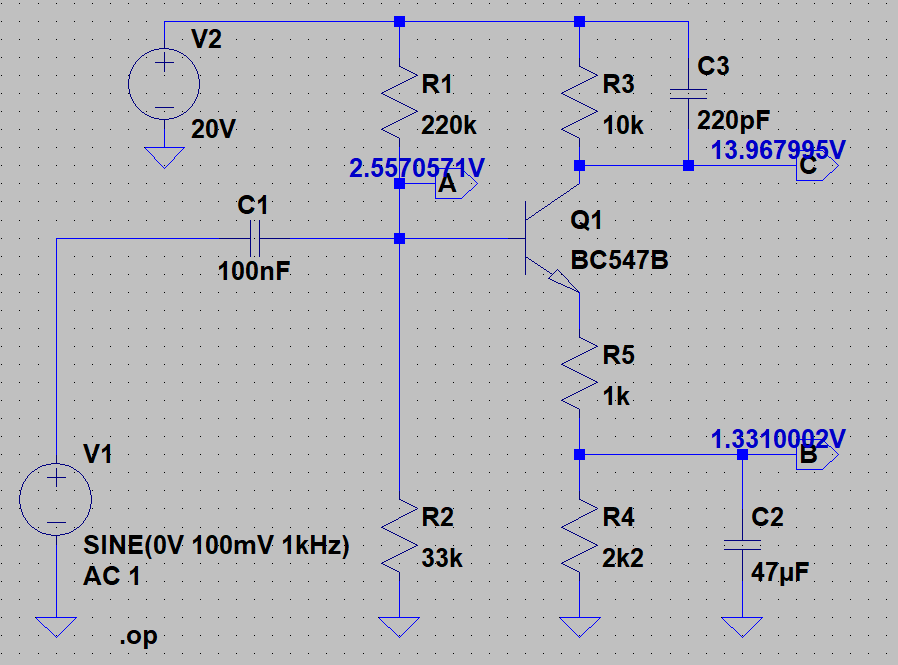
\includegraphics[width=0.7\linewidth]{321.PNG}
                \caption{Aufbau der Schaltung zum Bestimmen der Arbeitspunkte}
            \end{figure}

            Durch das Simulieren mit dem Befehl $DC op pnt.$ ergeben sich folgende Werte für die Gleichspannung.
            \begin{enumerate}
                \item A=2,557V
                \item B=1,332V
                \item C=13,968V
            \end{enumerate}

            \newpage
        \subsection{Eingangs- und Ausgangswiderstand}
            Zum Bestimmen des Ausgangs- und Eingangswiderstandes wird die Schaltung wie folgt aufgebaut. Dabei ist zu beachten, dass der Koppelkondensator C1 überbrückt werden muss.

            \begin{figure}[h!]
                \centering
                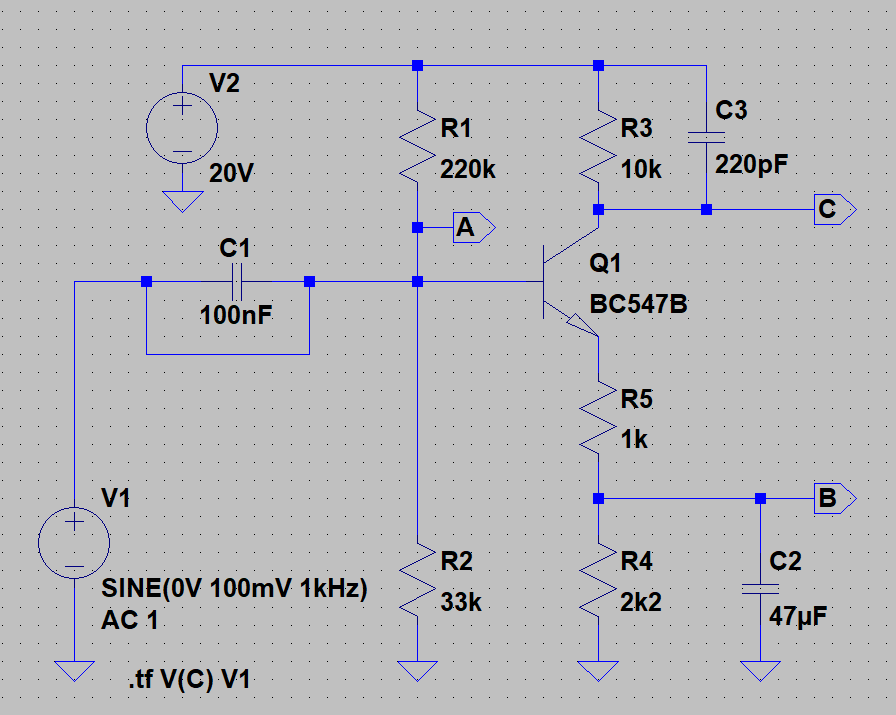
\includegraphics[width=0.7\linewidth]{322.PNG}
                \caption{Aufbau der Schaltung zum Bestimmen des Eingangs- und Ausgangswiderstandes}
            \end{figure}

            Die Simulation wird mit dem Befehl $DC Transfer$ ausgeführt. Dabei ist für Output V(C) und für Source V1 einzusetzen. Für den Eingangs- und Ausgangswiderstand der Schaltung ergeben sich folgende Werte.

            \begin{figure}[h!]
                \centering
                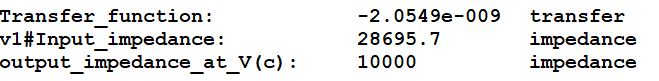
\includegraphics[width=0.7\linewidth]{3221.PNG}
                \caption{Aufbau der Schaltung zum Bestimmen der Arbeitspunkte}
            \end{figure}

            \newpage
        \subsection{Frequenzgang}
            \label{Frequenz}
            Um den Frequenzgang der Schaltung zu bestimmen wird der Befehl $AC Analysis$ eingegeben. Der Start der Frequenz beginnt bei 20 Hz und endet bei 200kHz. Der Type of sweep ist mit Decade zu wählen und die Anzahl der Punkte pro Decade wird mit 100 simuliert.

            \begin{figure}[h!]
                \centering
                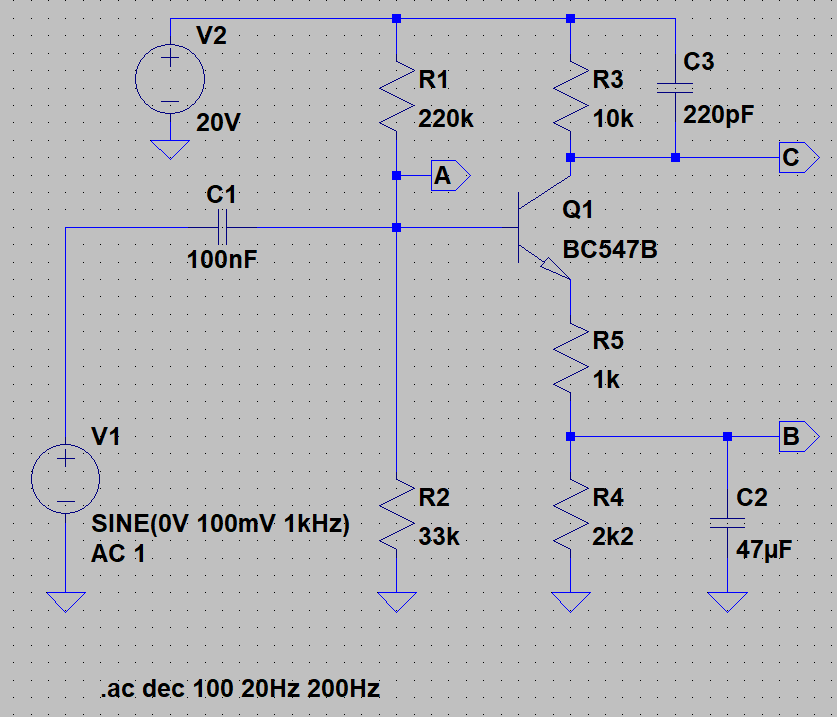
\includegraphics[width=0.7\linewidth]{323.PNG}
                \caption{Aufbau der Schaltung zum Bestimmen des Frequenzganges}
            \end{figure}

            Zum bestimmen der oberen und unteren Grenzfrequenz muss der Tiefpass und der Hochpass ermittelt werden. Den Hochpass, also die untere Grenzfrequenz lässt sich am Punkt A ermitteln. Der Tiefpass, also die obere Grenzfrequenz lässt sich am Punkt C bestimmen. Dabei ist zu beachten das die Grenzfrequenzen immer bei -3 dB liegen.

            Am Punkt A ergibt sich folgender Graph.
            \begin{figure}[h!]
                \centering
                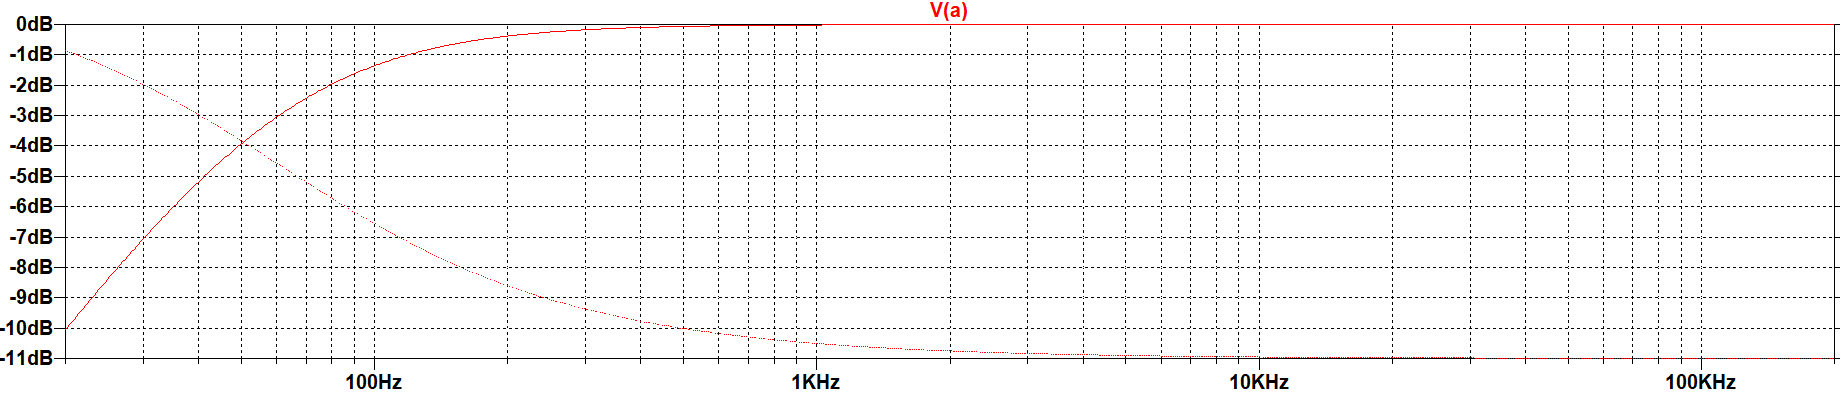
\includegraphics[width=\linewidth]{3232.PNG}
                \caption{Darstellung vom Hochpass}
            \end{figure}
            Die untere Grenzfrequenz liegt in diesem Graphen bei -3 dB was  \underline{60 Hz} entspricht.
            Am Punkt C ergibt sich dieser Graph \figref{tief}.
            
            \begin{figure}[h!t]
                \centering
                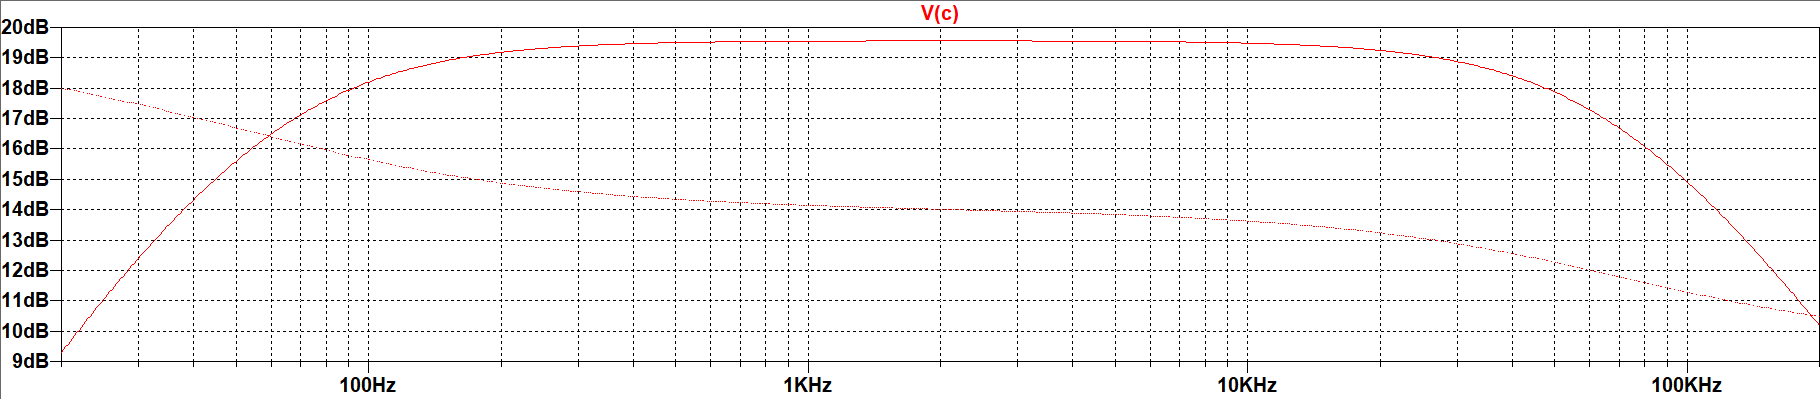
\includegraphics[width=\linewidth]{3233.PNG}
                \caption{Darstellung des Tiefpass}
                \label{tief}
            \end{figure}
            \par
            Für eine mittlere Frequenz ergibt sich eine Wert von \(\bar{f} = \SI{19,566}{\dB}\) und für die untere und obere Grenzfrequenz wird von LTSpice die Courser-Funktion genutzt \figref{grenzfrequenz} 
            Hierraus kann man ablesen das die untere Grenzfrequenz, angegeben im Bereich von Cursor 1 eine Frequenz von \SI{60.729}{\Hz} hat. Der Bereich von Cursor 2 gibt die obere Grenzfrequenz an mit \SI{70,380}{\Hz}.
            \begin{figure}[h!t]
                \centering
                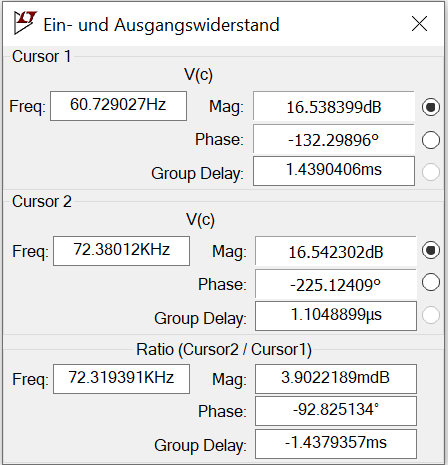
\includegraphics[scale=0.7]{cursor.PNG}
                \caption{Simulation der unteren und oberen Grenzfrequenz}
                \label{grenzfrequenz}
            \end{figure}


            \newpage
        \subsection{Temperaturabhängigkeit des Arbeitspunktes}
            Zum bestimmen der Temperaturabhängigkeit am Arbeitspunkt C muss die Simulation mit $DC sweep$ ausgeführt werden. Für den $name of first source of sweep$ wird $TEMP$ eingetragen. Für $Type of sweep$ wird $linear$ eingetragen und es wird das Intervall zwischen 0 und 100 simuliert. Mit folgender Schaltung wird simuliert.

            \begin{figure}[h!]
                \centering
                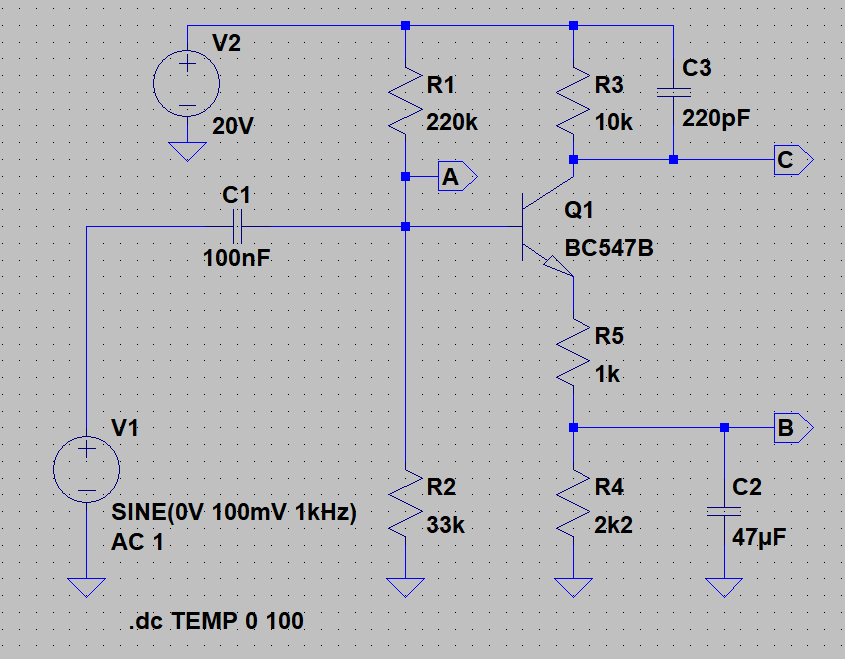
\includegraphics[width=0.7\linewidth]{324.PNG}
                \caption{Aufbau der Schaltung zum Bestimmen der Temperaturabhängigkeit}
            \end{figure}

            Folgender Graph ergibt sich durch die Simulation.
            \begin{figure}[h!]
                \centering
                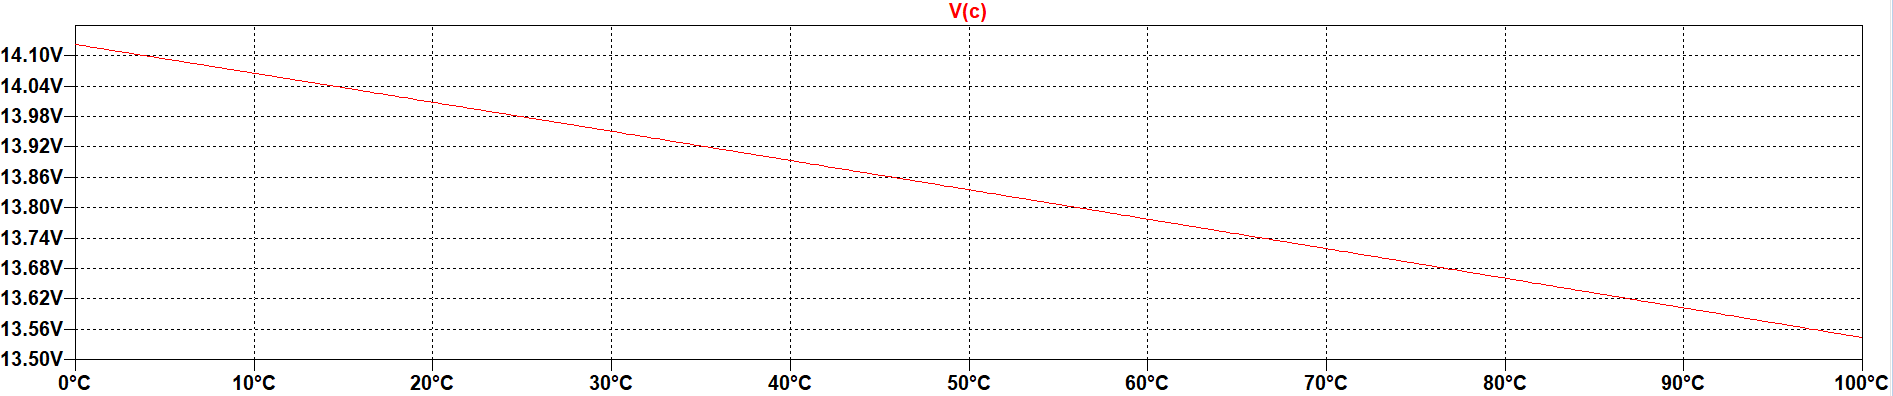
\includegraphics[width=\linewidth]{3241.PNG}
                \caption{Graph der Temperaturabhängigkeit am Arbeitspunkt C}
            \end{figure}


            \newpage
        \subsection{Großsignalbetrieb}
            Zum Bestimmen der noch unverzerrten Amplitude für das Eingangs- und Ausgangssignal wird der Befehl $Transistient$ im Intervall von 0ms bis 5ms für die Simulation verwendet. 

            \begin{figure}[h!]
                \centering
                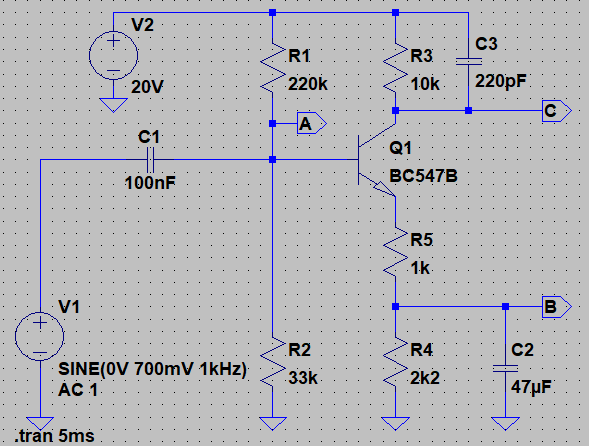
\includegraphics[width=0.7\linewidth]{325.PNG}
                \caption{Schaltung zur Bestimmung des unverzerrten Ausgangs- Eingangssignals}
            \end{figure}

            Dabei wurde die Eingangsspannung von 100mV in 100mV schritten erhöht bis diese sich bei 800mV verzerrt hat.
            \begin{figure}[h!]
                \centering
                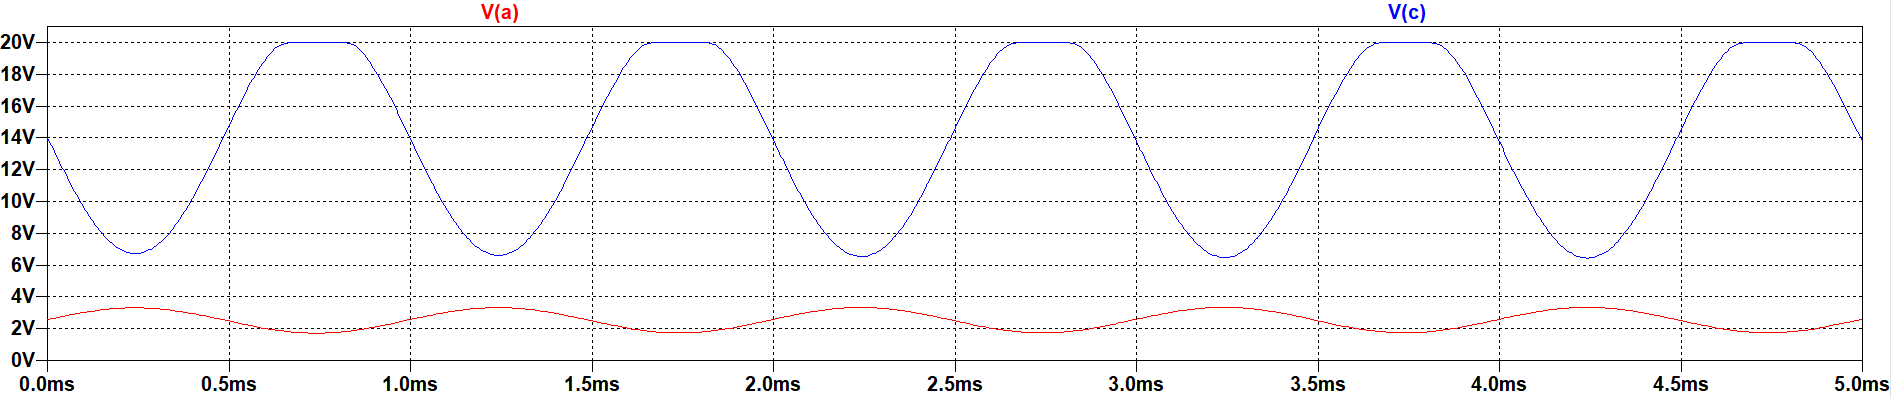
\includegraphics[width=\linewidth]{3251.PNG}
                \caption{Verzerrung des Ausgangssignals bei 800mV}
            \end{figure}
            Es ist zu erkennen, das die Amplitude bei 800mV sich im oberen Bereich verzerrt, da diese keinen Wert über 20 V erreichen kann. Dies bedeutet das eine Eingangsspannung von ungefähr 700 mV ohne einer daraus folgenden Verzerrung angelegt werden kann.


            \newpage
        \subsection{Einfluss der Tastkopfimpedanz}
            Nun wird wie in 3.2.3 Frequenzgang simuliert, mit dem Unterschied, dass am Ausgang C eine Tastkopfimpedanz zwischengeschaltet wird. Diese besteht aus einem Widerstand R mit $1M\Omega$ und einem Kondensator C mit $120pF$ ~\cite{tastkopf_standard}.

            \begin{figure}[h!]
                \label{fig:tast}
                \centering
                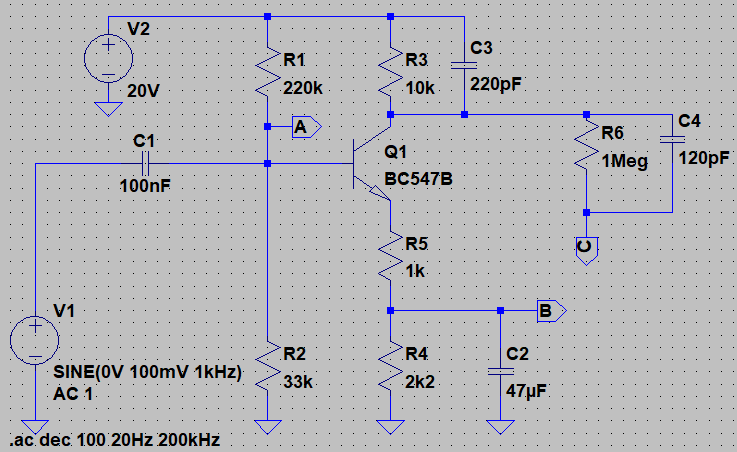
\includegraphics[width=0.7\linewidth]{326.PNG}
                \caption{Aufbau des Schaltbildes mit Tastkopfimpedanz}
            \end{figure}

            Durch die selben Simulationsanweisungen wie bei \ref{Frequenz} erhalten wir folgenden Graphen.

            \begin{figure}[h!]
                \centering
                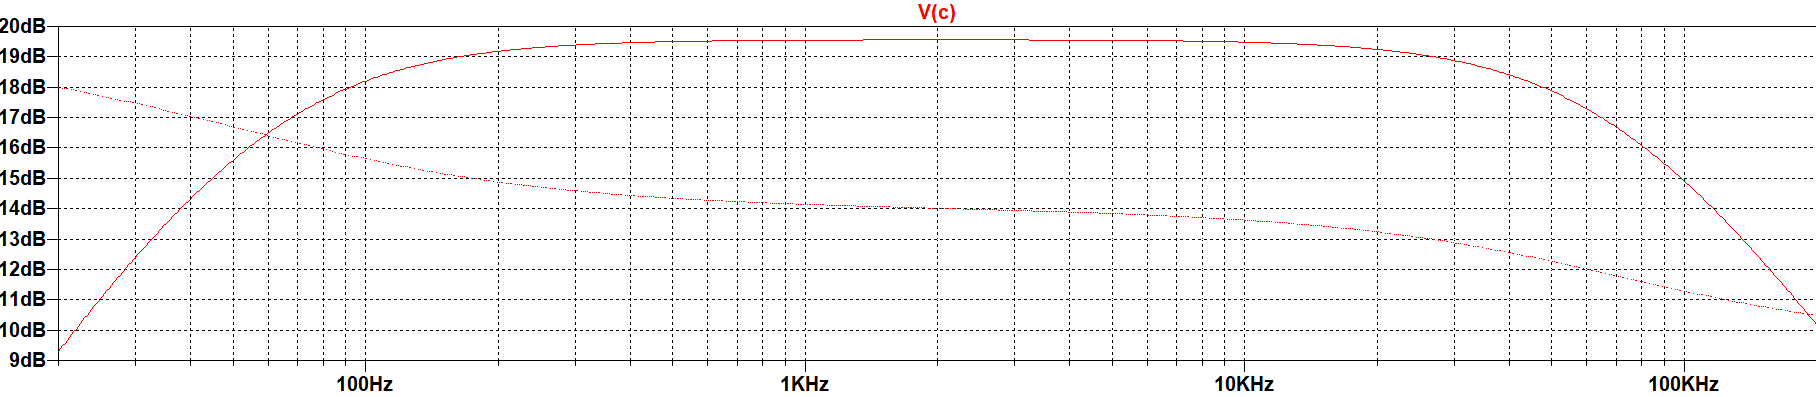
\includegraphics[width=\linewidth]{3261.PNG}
                \caption{Graph für den Frequenzgang mit Tastkopfimpedanz}
            \end{figure}
            Der Graph ohne Tastkopfimpedanz \ref{Frequenz} und mit Tastkopfimpedanz am Punkt C verändern sich jedoch nicht.

